%-----------------------------------------------------------------------------
% Schriftgröße, Layout, Papierformat, Art des Dokumentes
%-----------------------------------------------------------------------------
\documentclass[12pt,					% Grundschriftgöße
							 oneside,			% einseitiges Dokument
							 a4paper,			% Papiergröße
							 halfparskip,		% Einzug bei einem Absatz
							 liststotoc,			% Verzeichniss (Abbildungen erc.) in das Inhaltverzeichnis
							 bibtotoc,			% Literaturverzeichnis ins Inhaltverzeichnis
							 fleqn,				% Mathematische Formeln linksbündig darstellen
							 pointlessnumbers]	% Punkt am Ende der Nummerierung des Inhaltsverzeichnisses entfernen
							 {scrreprt}

%-----------------------------------------------------------------------------
% Konstanten festlegen
%-----------------------------------------------------------------------------
\newcommand{\VerfasserA}{Nicole Goldmann}
\newcommand{\GeburtstagA}{20. August 1997}
\newcommand{\GeburtsortA}{Herbolzheim}
\newcommand{\VerfasserB}{Stefanie Weidemann}
\newcommand{\GeburtstagB}{25. August 1995}
\newcommand{\GeburtsortB}{Anklam}
\newcommand{\Titel}{Webapp für Studiende des Studienganges AIMMT}
\newcommand{\Betreuer}{Prof. Dr.-Ing. Herbert Litschke}
\newcommand{\blankpage}{
	\newpage
	\thispagestyle{empty}
	\mbox{}
	\newpage
}

%-----------------------------------------------------------------------------
% verwendete Pakete
%-----------------------------------------------------------------------------
\usepackage[T1]{fontenc}				% Wahl des Fonts, bzw. der Kodierung
\usepackage[utf8]{inputenc}			% Zeichkodierung , Umlaute erlauben
\usepackage[english,ngerman]{babel}		% neue deutsche Rechtschreibung verwenden
\usepackage{graphicx}					% erm�glicht das Einbinden von Grafiken, sehr wichtig!
\usepackage{fancyhdr}					% f�r formatierte Kopf- und Fu�zeilen
\usepackage{setspace}					% Package zum Kontrollieren von Leerr�umen
\usepackage{subfigure}					% erweiterte Darstellung von Bildern
\usepackage{listings}					% M�glickeit zum Anzeigen von Quelltexten
\usepackage{color,moreverb}				% Farben
\usepackage{lmodern}					% bietet neuere Schriften, sieht besser aus im Acrobat Reader
\usepackage{amsmath,amssymb}			% erweiteter Formelsatz und zus�tzliche Mathe-Symbole
\usepackage{booktabs}					% professionelle, typographisch richtige Tabellen
\usepackage{cite}						% f�r LibTex
%\usepackage{shortvrb}					% f�r Quellcode mit \begin{verbatim}
\usepackage[binary-units=true]{siunitx}	% Darstellung von Si-Einheiten
\usepackage{enumitem}					% custom itemiziation
\usepackage{textcomp}
\usepackage{url}
%-----------------------------------------------------------------------------
% Fu�notennummerierung nicht f�r jedes kapitel zur�cksetzen
%-----------------------------------------------------------------------------
\usepackage{chngcntr}
\counterwithout{footnote}{chapter}

%-----------------------------------------------------------------------------
% Einstellungen der Seitenr�nder
%-----------------------------------------------------------------------------
\usepackage[left=3cm,						% linker Rand
						right=3cm,			% rechter Rand
						top=1.5cm,			% oberer Rand
						bottom=1.5cm,		% unterer Rand
						includeheadfoot,	% bezieht die Kopf- und Fu�zeile mit ein
						bindingoffset=0cm]	% Bundsteg
						{geometry}

%-----------------------------------------------------------------------------
% Daten f�r die Titel des Artikels
%-----------------------------------------------------------------------------
\title{Semesterarbeit}
\author{\VerfasserA, VerfasserB}
\date{\today{}}

%-----------------------------------------------------------------------------
% Metadaten in pdf einf�gen
%-----------------------------------------------------------------------------
\usepackage[pdftex,
						pdfauthor={\VerfasserA, VerfasserA},					% Name des Autors
						pdftitle={\Titel},										% Name der Arbeit
						pdfcreator={MiKTeX, LaTeX with hyperref and KOMA-Script},	% Von was erzeugt
						%pdfsubject={Praktikumsbericht},							% Was f�r eine Arbeit ist es
						pdfkeywords={\Titel},
						plainpages=false,
						hypertexnames=false,
						pdfpagelabels]{hyperref}

%-----------------------------------------------------------------------------
% Schriftarten anpassen
%-----------------------------------------------------------------------------
\setkomafont{sectioning}{\rmfamily\bfseries}			% Titelzeilen
\setkomafont{caption}{\small}							% Schrift f�r Caption
\setkomafont{captionlabel}{\sffamily\bfseries\small}	% Schrift f�r 'Abbildung'
\setkomafont{chapterentry}{\small\bfseries}				% Schrift f�r Inhaltsverzeichnis
\setkomafont{chapter}{\large\bfseries}					% Schrift f�r Kapitel
\setkomafont{section}{\normalsize}						% Schrift f�r Section
\setkomafont{subsection}{\normalsize}					% Schrift f�r Subsection

%-----------------------------------------------------------------------------
% "Quellcode"-Unterschrift von Listing in Quellcode umbennen
%-----------------------------------------------------------------------------
\addto{\captionsngerman}{\renewcommand*{\lstlistingname}{Quellcode}}

%-----------------------------------------------------------------------------
% Farbe f�r Links in PDF-Dokumenten definieren
%-----------------------------------------------------------------------------
\definecolor{LinkColor}{rgb}{0,0,0}				% Festlegen einer neuen Farbe

\hypersetup{colorlinks=true,					% farbliche Links
						breaklinks=true,		% Zeilenumbruch erlauben
						linkcolor=black,		% Farbe f�r interne Links
						citecolor=black,		% Farbe f�r Links zum Literaturverzeichnis
						filecolor=LinkColor,	% Farbe f�r externe Dateilinks
						menucolor=LinkColor,	%
						urlcolor=LinkColor}		% Farbe f�r externe Links
						
%-----------------------------------------------------------------------------
% Definition f�r Quelltextlistings
%-----------------------------------------------------------------------------
\lstloadlanguages{C}

\definecolor{lbcolor}{gray}{0.95}			% Farbe f�r den Hintergrund definieren				
\definecolor{darkblue}{rgb}{0,0,.6}		% Farbe f�r Schl�sselw�rter
\definecolor{darkred}{rgb}{.6,0,0}		% Farbe f�r Strings
\definecolor{darkgreen}{rgb}{0,.6,0}		% Farbe f�r Kommentare

\lstset{language=C,								% Programmiersprache der Listings
				alsolanguage=Matlab,			% alternative Programmiersprache der Listings
				frame=none,								% keinen Rahmen
				frameround=ffff,					% wenn ein Rahmen dargestellt werden soll, sind die Ecken spitz
				captionpos=b,							% Position der Benennung
				numbers=left,							% Zeilennummern links angeben
				stepnumber=1,							% in welchem Abstand sollen Zeilennummern angeben werden (1 2 3..)
				numbersep=3pt,						% Abstand zwischen Nummerierung und Listing
				numberstyle=\tiny,				% gr�sse der Nummern
				breaklines=true,					% Zeilenumbruch zulassen
				breakautoindent=true,
				postbreak=\space,
				tabsize=4,								% Tabulator auf 4 setzen
				escapechar=\$,
				basicstyle=\scriptsize\ttfamily,
				keywordstyle=\color{darkblue}\bfseries\ttfamily,	% Darstellung der Schl�sselw�rter
				stringstyle=\ttfamily\color{darkred},  						% Darstellung der Strings
				commentstyle=\itshape\color{darkgreen},						% Darstellung der Kommentare
				showspaces=false,					% leerzeichen nicht anzeigen
				showstringspaces=false,		% keine Leerzeichen bei Strings anzeigen
				xleftmargin=.52cm,
				xrightmargin=.52cm,				
				backgroundcolor=\color{lbcolor}}	% Hintergrundfarbe des Listings
				
%-----------------------------------------------------------------------------
% Kopf- und Fusszeile bestimmen
%-----------------------------------------------------------------------------
\pagestyle{fancy}	
\fancyhf{}												% alle Felder l�schen
\fancypagestyle{plain}{}

% Kopfzeile rechts bzw. au�en
\fancyhead[R]{\nouppercase{\leftmark}}
% Linie oben
\renewcommand{\headrulewidth}{0.5pt}
% Fu�zeile rechts bzw. au�en
\fancyfoot[R]{\thepage}
%-----------------------------------------------------------------------------

%-----------------------------------------------------------------------------
% Begin des Dokuments
%-----------------------------------------------------------------------------
\begin{document} 						% Beginn des Dokumentes

	\renewcommand\lstlistingname{Code}
	\renewcommand\lstlistlistingname{Codeverzeichnis}
	
	%% Titel
	\begin{titlepage}
		\setlength\headsep{-5mm}
		\begin{figure}[!h]
			\begin{minipage}{0.8\textwidth}
				\textbf{Hochschule Wismar} \\
				University of Applied Sciences \\
				Technology, Business and Design \\
				Fakultät für Ingenieurwissenschaften, Bereich EuI \\
			\rule{\textwidth}{0.5pt}
			\end{minipage}
			\begin{minipage}[r]{0.1\textwidth}
				\begin{flushright}
					
\includegraphics[height=6\baselineskip]{pictures/HS-Wismar_Logo-FIW_2010-01.jpg}
				\end{flushright}
			\end{minipage}
		\end{figure}
		\vspace*{6cm}
		\begin{center}
			\Huge
			\textbf{Projektarbeit} \\
			\vspace{2cm}
			\large \Titel
			\begin{table*}[b]
				\begin{tabular}{rl}
					Gedruckt am: & \today \\
					\\
					von: & \VerfasserA \\
					& geboren am \GeburtstagA \\
					& in \GeburtsortA \\
					\\
					von: & \VerfasserB \\
					& geboren am \GeburtstagB \\
					& in \GeburtsortB \\
					\\
					Betreuer: & \Betreuer \\

				\end{tabular}
			\end{table*}
		\end{center}
	\end{titlepage}

	\onehalfspacing 					% 1 1/2-zeilig (package 'setspace')
	
	%\blankpage	%leeres Blatt zwischen Deckblatt und Inhaltsverzeichnis	
	%-----------------------------------------------------------------------------
	% Inhaltsverzeichnis
	%-----------------------------------------------------------------------------	
	\pdfbookmark[1]{Inhaltsverzeichnis}{toc}	% Inhaltsverzeichnis zu den Lesezeichen hinzufügen
	%\singlespacing 						% 1-zeilig
	\tableofcontents					% Inhaltverzeichnis einf�gen
	%\onehalfspacing 					% 1 1/2-zeilig (package 'setspace')

	%-----------------------------------------------------------------------------
	% Hauptteil
	%-----------------------------------------------------------------------------	

%\begin{itemize}
%\item \textit{/ig-hashtag-search root edge:} über die Hashtag-ID
%\item \textit{/hashtag node:} ein bestimmter Hashtag
%\item \textit{/hashtag/top-media edge:} Fotos und Videos unter einem bestimmten Hashtag
%\item \textit{/hashtag/recent-media edge:} kürzlich veröffentlichte Fotos und Videos unter einem bestimmten Hashtag
%\item \textit{/user/recently searched hashtags edge:} gesuchte Hashtags eines Business Account in einer Woche
%\end{itemize}

%\cite{insta}


%\begin{figure}[h]%riesen Graphen
%	\centering
%	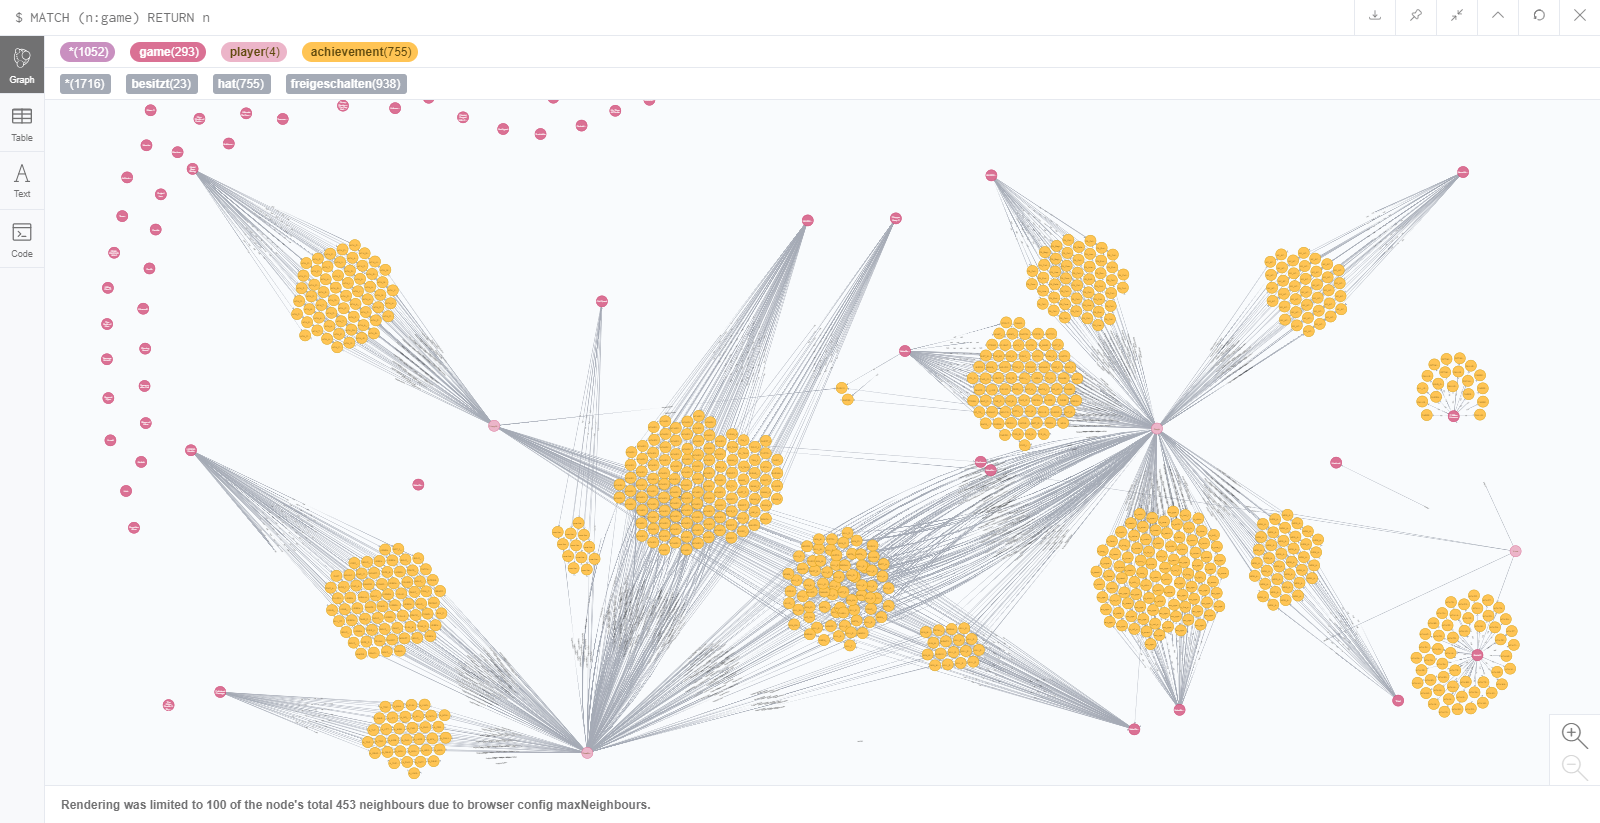
\includegraphics[width=1\textwidth]{pictures/Datenbank_v2.png}
%	\label{Knoten_DB}
%\end{figure}

\newpage
\chapter*{Aufgabenstellung:}

\newpage

\chapter{Einleitung}

\chapter{Untersuchung der Hochschul Website}	
Studenten die Informationen zu ihrem Studiengang suchen brauchen teilweise sechs Klicks um von der Startseite der HS Wismar zur Semsterübersicht (AIMMT) zu gelangen. Innerhalb dieser Seiten gibt es einige Unstimmigkeiten und fehlerhaftes Fehlerhaftes Verhalten, welches im folgendem näher erläutert wird.
		\section{Analyse des Ist-Zustandes}
		Die Hochschulwebsite hat einen großen allgemeinen Teil der Informationen über die Hochschule enthält und hat Verlinkungen zu den drei Fakultätsseiten. Da die entwickelte Webanwendung für Studierende des Studiengangs Angewandte Informatik und Multimendiatechnik gedacht ist wird an dieser Stelle nur die Fakultätsseite der Ingenieurstechnik bzw. des Bereiches Elektrotechnik und Information.
		
		In der oberen Navigationsleiste gibt es nicht eindeutig erkennbare Icons für den Schnelleinstig und Informationen. Werden diese angeklickt, klappt sich ein Panel nach oben aus. Die obere Navigationsleiste ist nicht fixiert. Der Footer ist sehr groß und enthält teilweise die selben Verlinkungen wie in der Seitennavigation oben. Auf der Seite der Semsterübersicht gib es eine Akkordeonmenü welches nicht an allen Punkten anklickbar ist. Dieses Menü enthält ein Pfeil-Icon nach unten zeigend, welches dem User sugerriert das sich hinter dem Icon mehr Informationen enthalten.  Dieses Icon ist aber nicht anklickbar. Die Pfeil-Icons gibt es auf der gesamten Website als wiederkehrendes Symbol für Verlinkungen. Auf den Informationsseiten werden diese Icons allerdings auch als Auflistungszeichen verwendet. Weiterhin gibt es viel zu viele Querverweise. Beispielsweise auf einer Modulübersichtsseite gibt es Verlinkungen zu weiteren Studiengängen die dieses Modul besuchen, weitere Module die der/die Professor |in unterrichtet, die Forschungsthemen, Thesenthemen, und Jobs die der/die Professor|in anbietet. Diese Informationen gibt als sowohl auf der Modulübersicht als auch auf der persönlichen Seite der/des Professor|in. Der User wird überfordert, da zu viele Informationen gegeben werden. Desweiteren fehlt die Auflistung der Wahlpflichtmodule. Diese müssen umständlich im Modulhandbuch gesucht werden. 
		
		\section{Festlegung Systemanforderung}
		Die Hochschulwebsite ist sowohl für Studieninterssierte, als auch für eingeschriebene Studierende konzipiert. Um schneller an die wichtigsten Informationen zu gelangen, soll die Anwendung nur für eingeschriebene Studierende des Studiengangs Angewandte Informatik und Multimediatechnik dienen. Weiterhin sollen nur die wichtigsten Information kurz und knapp dargestellt werden. Daher hat jede Seite ein klares Ziel.	So ergeben sich weniger Verlinkungen, sodass der User immer genau weiß wo er sich befindet. Die heutigen Studierenden gehören zur Generation Smartphone. Daher soll der Ansatz "mobile first" verfolgt werden.
	

\chapter{Grundlagen}				
		\section{Technische Grundlagen}
				\subsection{Programmiersprachen im Web}
				\subsection{Webapp}
				\subsection{Templates}
			
		\section{Responsive Webentwicklung}	
				\subsection{Positionierungseinheiten }
					px, prozent, vh, vw, em, rem ...
				\subsection{Umsetzung für verschiedene Displaygrößen}
				\subsection{click- vs Touchevents}
				\subsection{Elementanordnungen}
				


\chapter{Konzept}			
		\section{Use-Cases der Anwendung}	
		\section{Systementwurf}
		Die Webanwendung teilt sich in zwei Bereiche: Semesterübersicht und Professoren und Mitarbeiter Übersicht. Die Trennung erfolgt durch ein klares Farbschema. In der Semesterübersicht werden im ersten Schritt alle 7 Semester aufgelistet. Wählt der User ein Semester aus, sind alle Module die in dem ausgewählten Semester angeboten werden aufgelistet. Klickt der User auf ein Modul, erhält er weitere Informationen zu diesem Modul. Hier idt beschrieben welcher Professor|in unterrichtet, wie viele SWS, Credits und Inhalte dieses Modul bietet und welche Form die Prüfung hat. In der unteren Navigation kann der User jederzeit in die gewünschte Übersicht wechseln. In der Übersicht der Professoren, sind alle Professoren und Mitarbeiter die diesen Studiengang begleiten aufgelistet. Wählt der User eine Person aus, bekommt er wichtige Informationen wie Kontaktdaten (Büro, Telefonnummer, EMail) und eine Auflistung der Module die dieser unterrichtet. Bei den Mitarbeitern sind die Module aufgelistet die diese betreuen.
		
\chapter{Implementierung}  

	\section{...}



\chapter{Zusammenfassung und Ausblick}     


		
	
 	%-----------------------------------------------------------------------------
	% Literaturverzeichnis einfügen, 
	% Nutzung der BibTeX-Technologie --> literatur.bib 
	%-----------------------------------------------------------------------------
	
%	\bibliographystyle{unsrtdin}		%  Stil des Literaturverzeichnisses (hier nach DIN 1505)
%	\bibliography{literatur.bib}			% gibt Datei mit der Literatur an
	\nocite{*}						% damit alle in der DB enthaltende Einträge bearbeitet werden


\begin{thebibliography}{unsrt}
\bibitem{insta} \textit{Instagram API Platform}, 2019 Instagram\\
https://www.instagram.com/developer/ [08.06.2019]

\bibitem{twitter} \textit{Developer policy and terms} 2019 Twitter, Inc.\\
https://developer.twitter.com/ [08.06.2019]

\bibitem{steamallg} \textit{Steam}, Valve Corporation\\
https://store.steampowered.com/about/ [19.05.2019]

\bibitem{steam} \textit{Steam Web API}, Valve Developer Community, 2019 \\
https://developer.valvesoftware.com/wiki/Steam\_Web\_API [17.05.2019]

\bibitem{neo4j} \textit{Eine Graphendatenbank für alle}, Michael Hunger, 2014, Entwickler.Press, ISBN: 978-3-86802-128-0

\bibitem{kommneo4j} \textit{Diese Vorteile bieten Graphdatenbanken}, Kommentar von Stefan Kolmar, 2017\\
https://www.bigdata-insider.de/diese-vorteile-bieten-graphdatenbanken-a-615118/ [17.05.2019]


\end{thebibliography}	

	%-----------------------------------------------------------------------------
	% Verzeichnisse
	%-----------------------------------------------------------------------------
	\listoffigures						% Bildverzeichnis einfügen
%	\listoftables						% Tabellenverzeichnis einfügen
%	\lstlistoflistings					% Quellcodeverzeichnis einfügen

	%-----------------------------------------------------------------------------
	% Anhang
	%-----------------------------------------------------------------------------	
	\appendix
	% Auch hier sind Gliederungen aller \chapter, \section
	

	%-----------------------------------------------------------------------------
	% Selbstständigkeitserklärung
	%-----------------------------------------------------------------------------	
	\chapter*{Selbstständigkeitserklärung}
	\addcontentsline{toc}{chapter}{Selbstständigkeitserklärung}
	\rhead{Selbstständigkeitserklärung} % rechts oben in der Kopfzeile Chapter darstellen
	Hiermit erklären wir, dass wir die hier vorliegende Arbeit selbstständig,
	ohne unerlaubte fremde Hilfe und nur unter Verwendung der aufgeführten
	Hilfsmittel angefertigt haben.

	\begin{tabular}{p{6cm}p{7cm}}
		\\
  		\\
  		\\
  		\\
  		Ort, Datum & Unterschriften
	\end{tabular}
	
	
	
\end{document}							% Ende des Dokuments
%-----------------------------------------------------------------------------
